
\section{Projeto do motor}

Da metodologia e dos requisitos expostos na seção~\ref{sec:motor_project}, foi gerada a geometria do motor para impressão 3D. A figura~\ref{fig:internal_profile} mostra a seção longitudinal projetada para o motor. Destaca-se o grande volume da câmara em comparação com a tubeira, devido à necessidade de haver estagnação de um fluxo intenso (ver seção~\ref{sec:result_validation}).

\begin{figure}[htbp]
    \centering
    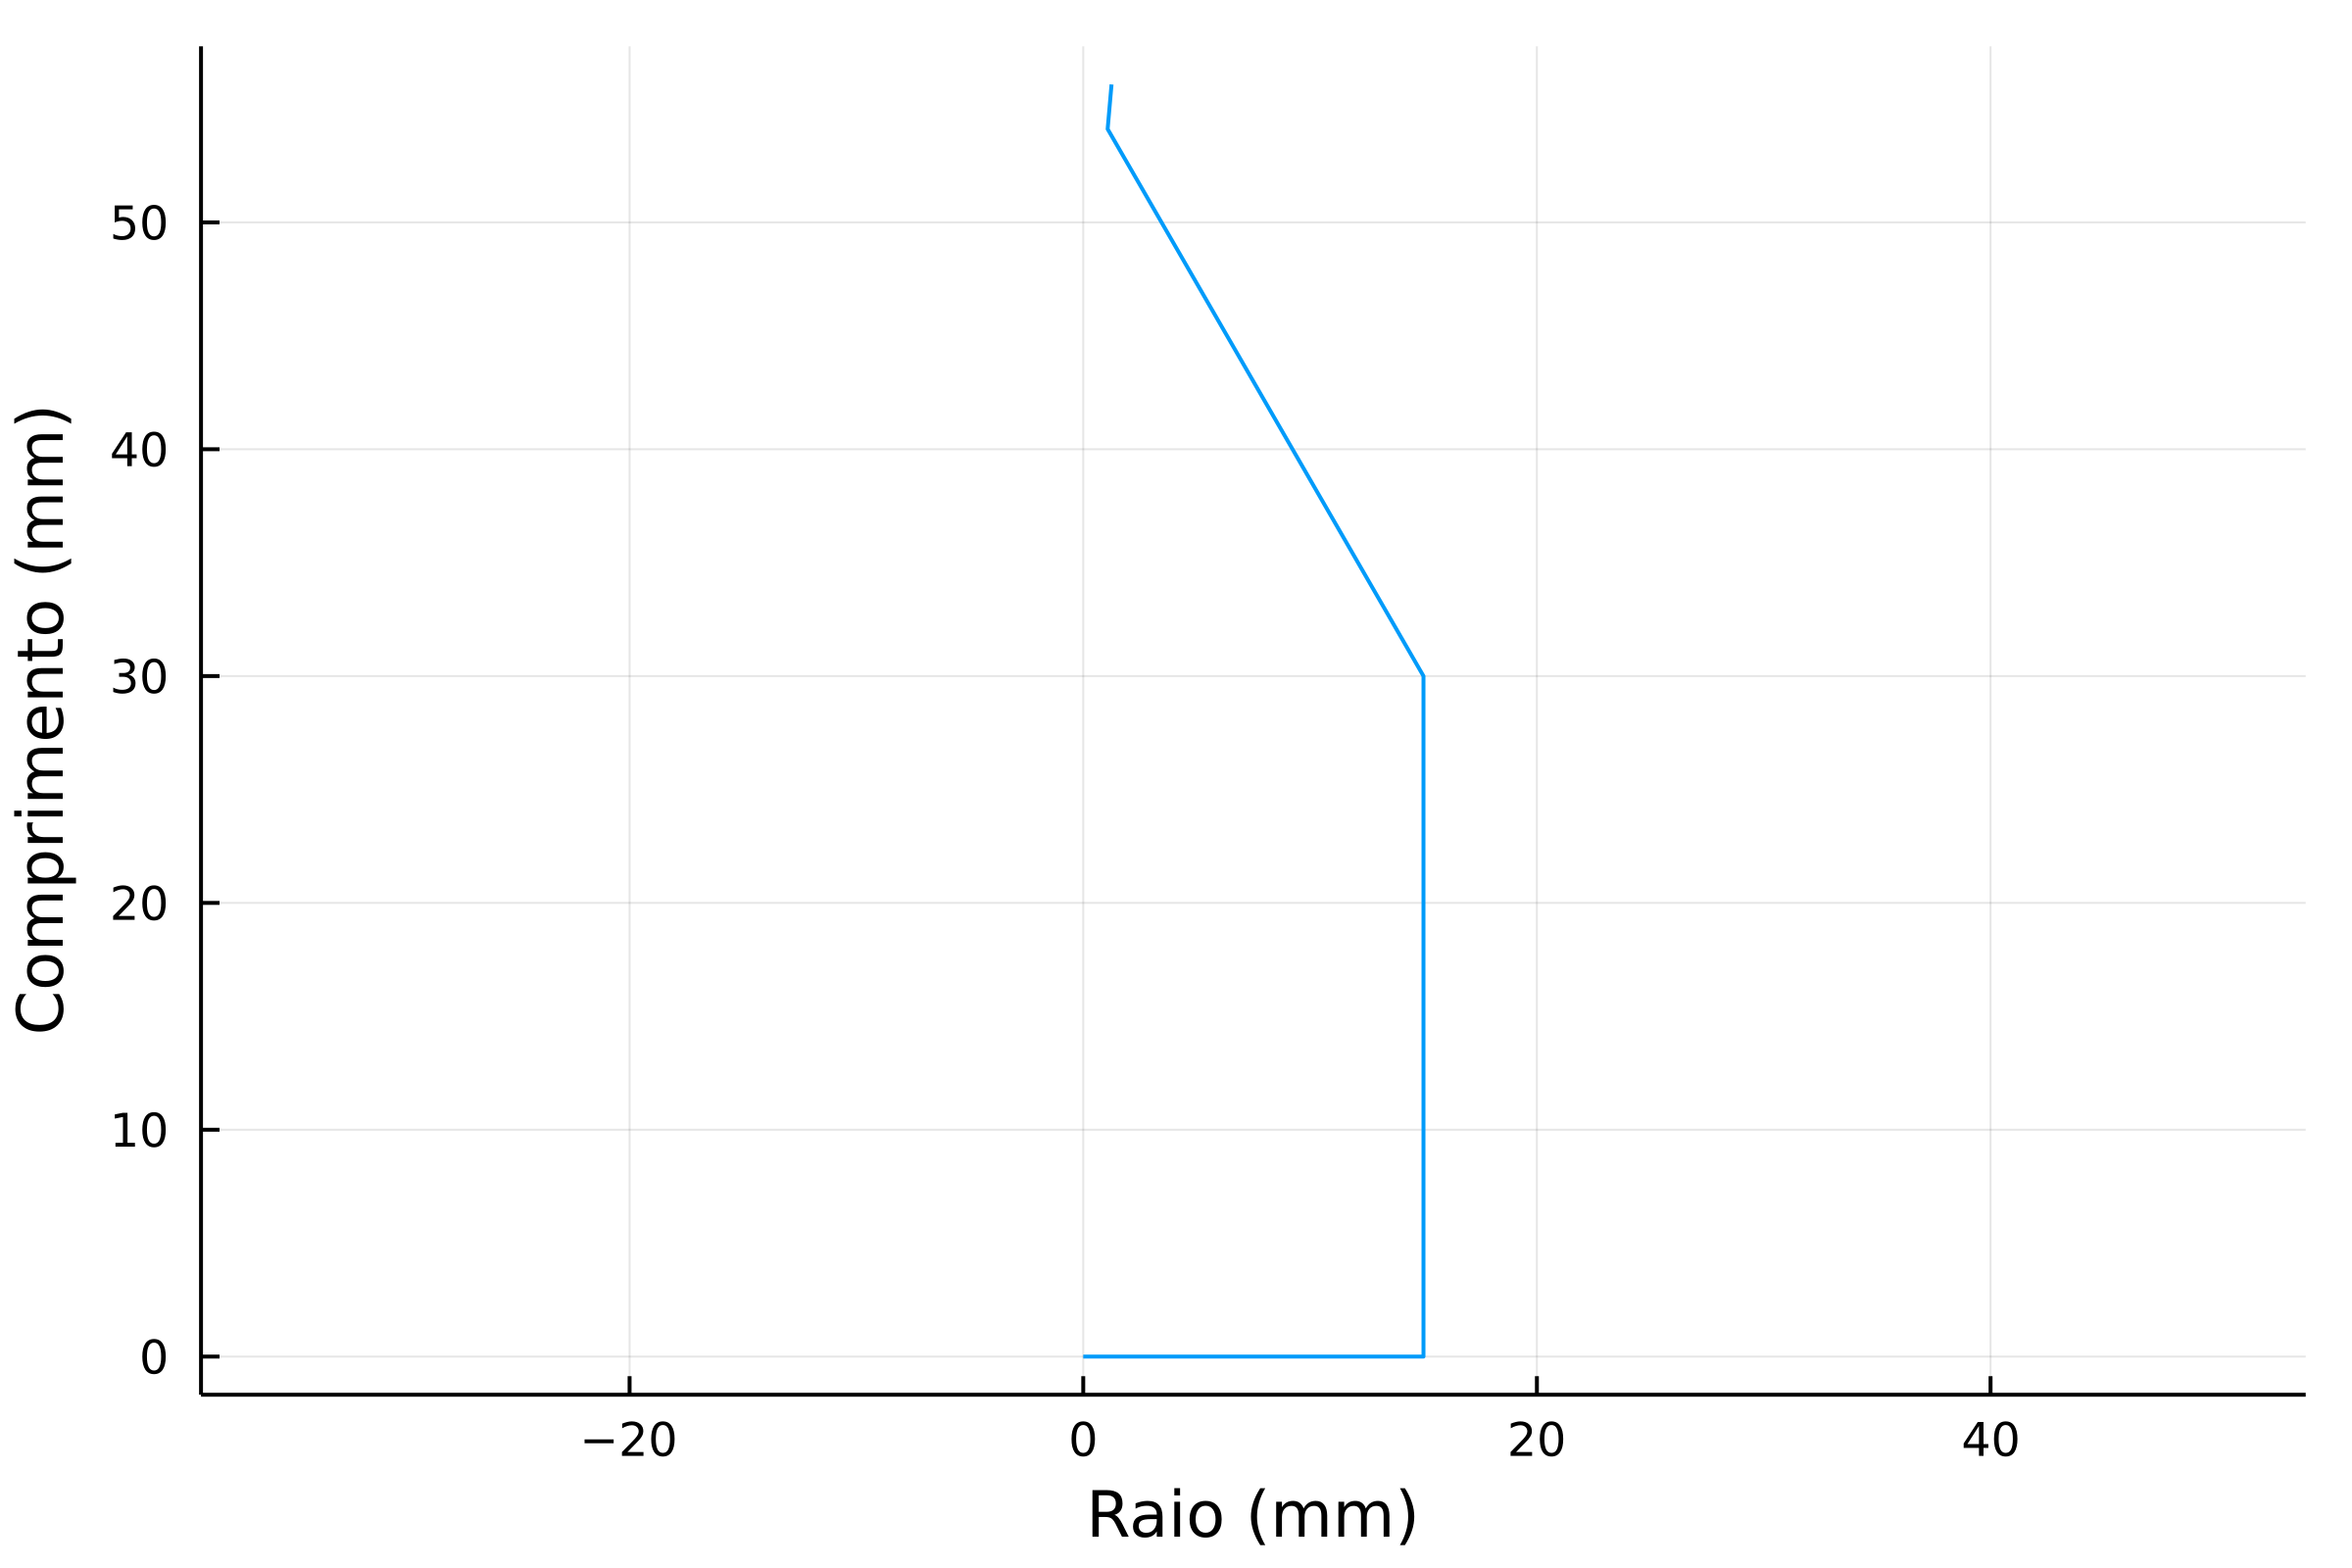
\includegraphics[width=\textwidth]{img/internal_profile.png}
    \caption{Perfil interno do motor projetado.}\label{fig:internal_profile}
\end{figure}

Os parâmetros propulsivos calculados para o motor foram:
\begin{itemize}
    \item \( \varepsilon = 1,35 \)
    \item \(C^* = 427,2\;\mathrm{m}\,\mathrm{s}^{-1}\)
    \item \(C_{F} = 1,10\)
\end{itemize}

Observa-se que o pequeno valor de razão de expansão é refletido na pequena tubeira exibida na figura~\ref{fig:internal_profile}. Foi obtido também um impulso específico de \(I_{sp} = 47,9s\) e um fluxo mássico de \(\dot{m} = 4,257\;\mathrm{g}\,\mathrm{s}^{-1}\). Devido à baixa energia do propelente, a velocidade característica do motor é bastante baixa, de modo que é necessário um fluxo mássico bastante elevado para a produção do empuxo requisitado. Isso é refletido no valor de impulso específico baixo. Ressalta-se também que o motor foi ajustado para operar à pressão ambiente, fator que limitou a razão de expansão e, portanto, o coeficiente de empuxo. 

O perfil da figura~\ref{fig:internal_profile} foi revolucionado para se obter uma geometria tridimensional, com superfícies planas externas adicionadas para facilitar a manufatura e a conexão com mangueiras de gás. Na figura~\ref{fig:3d_geom}, à esquerda, observa-se a geometria STL gerada em código para o motor. Foi adicionado um furo lateral para conexão com uma mangueira de alimentação, bem como quatro superfícies planas laterais para facilitar o manuseio e o apoio em morsas e outros equipamentos. À direita, observa-se o motor real construído \textcolor{red}{COLOCAR}. 

\begin{figure}[htbp]
    \centering
    \begin{subfigure}{0.49\textwidth}
        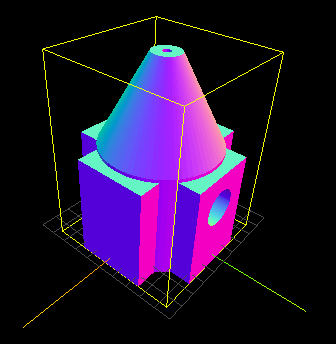
\includegraphics[width=\textwidth]{img/motor_stl.png}
        \caption{Geometria STL gerada para o motor.}
    \end{subfigure}
    \begin{subfigure}{0.49\textwidth}
        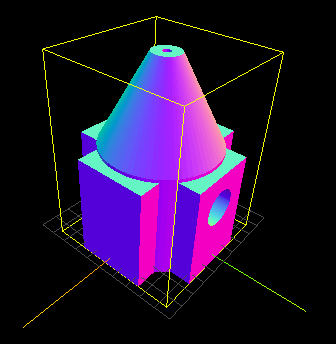
\includegraphics[width=\textwidth]{img/motor_stl.png}
        \caption{Motor impresso em 3D.}
    \end{subfigure}
    \caption{Geometria tridimensional do motor projetado.}
    \label{fig:3d_geom}
\end{figure}

\section{Validação do projeto do motor}\label{sec:result_validation}

A bancada de testes descrita na seção~\ref{sec:method_validation} gerou dados de empuxo para o motor e pressão estática e temperatura de câmara. A temperatura manteve-se bastante constante, próxima do valor especificado no requisito PRP-3, de modo que ela será tratada como constante e idêntica a este valor. O gráfico~\ref{fig:thrust_versus_p1} exibe as medidas de empuxo feitas em função da pressão de câmara medida.

\begin{figure}[htbp]
    \centering
    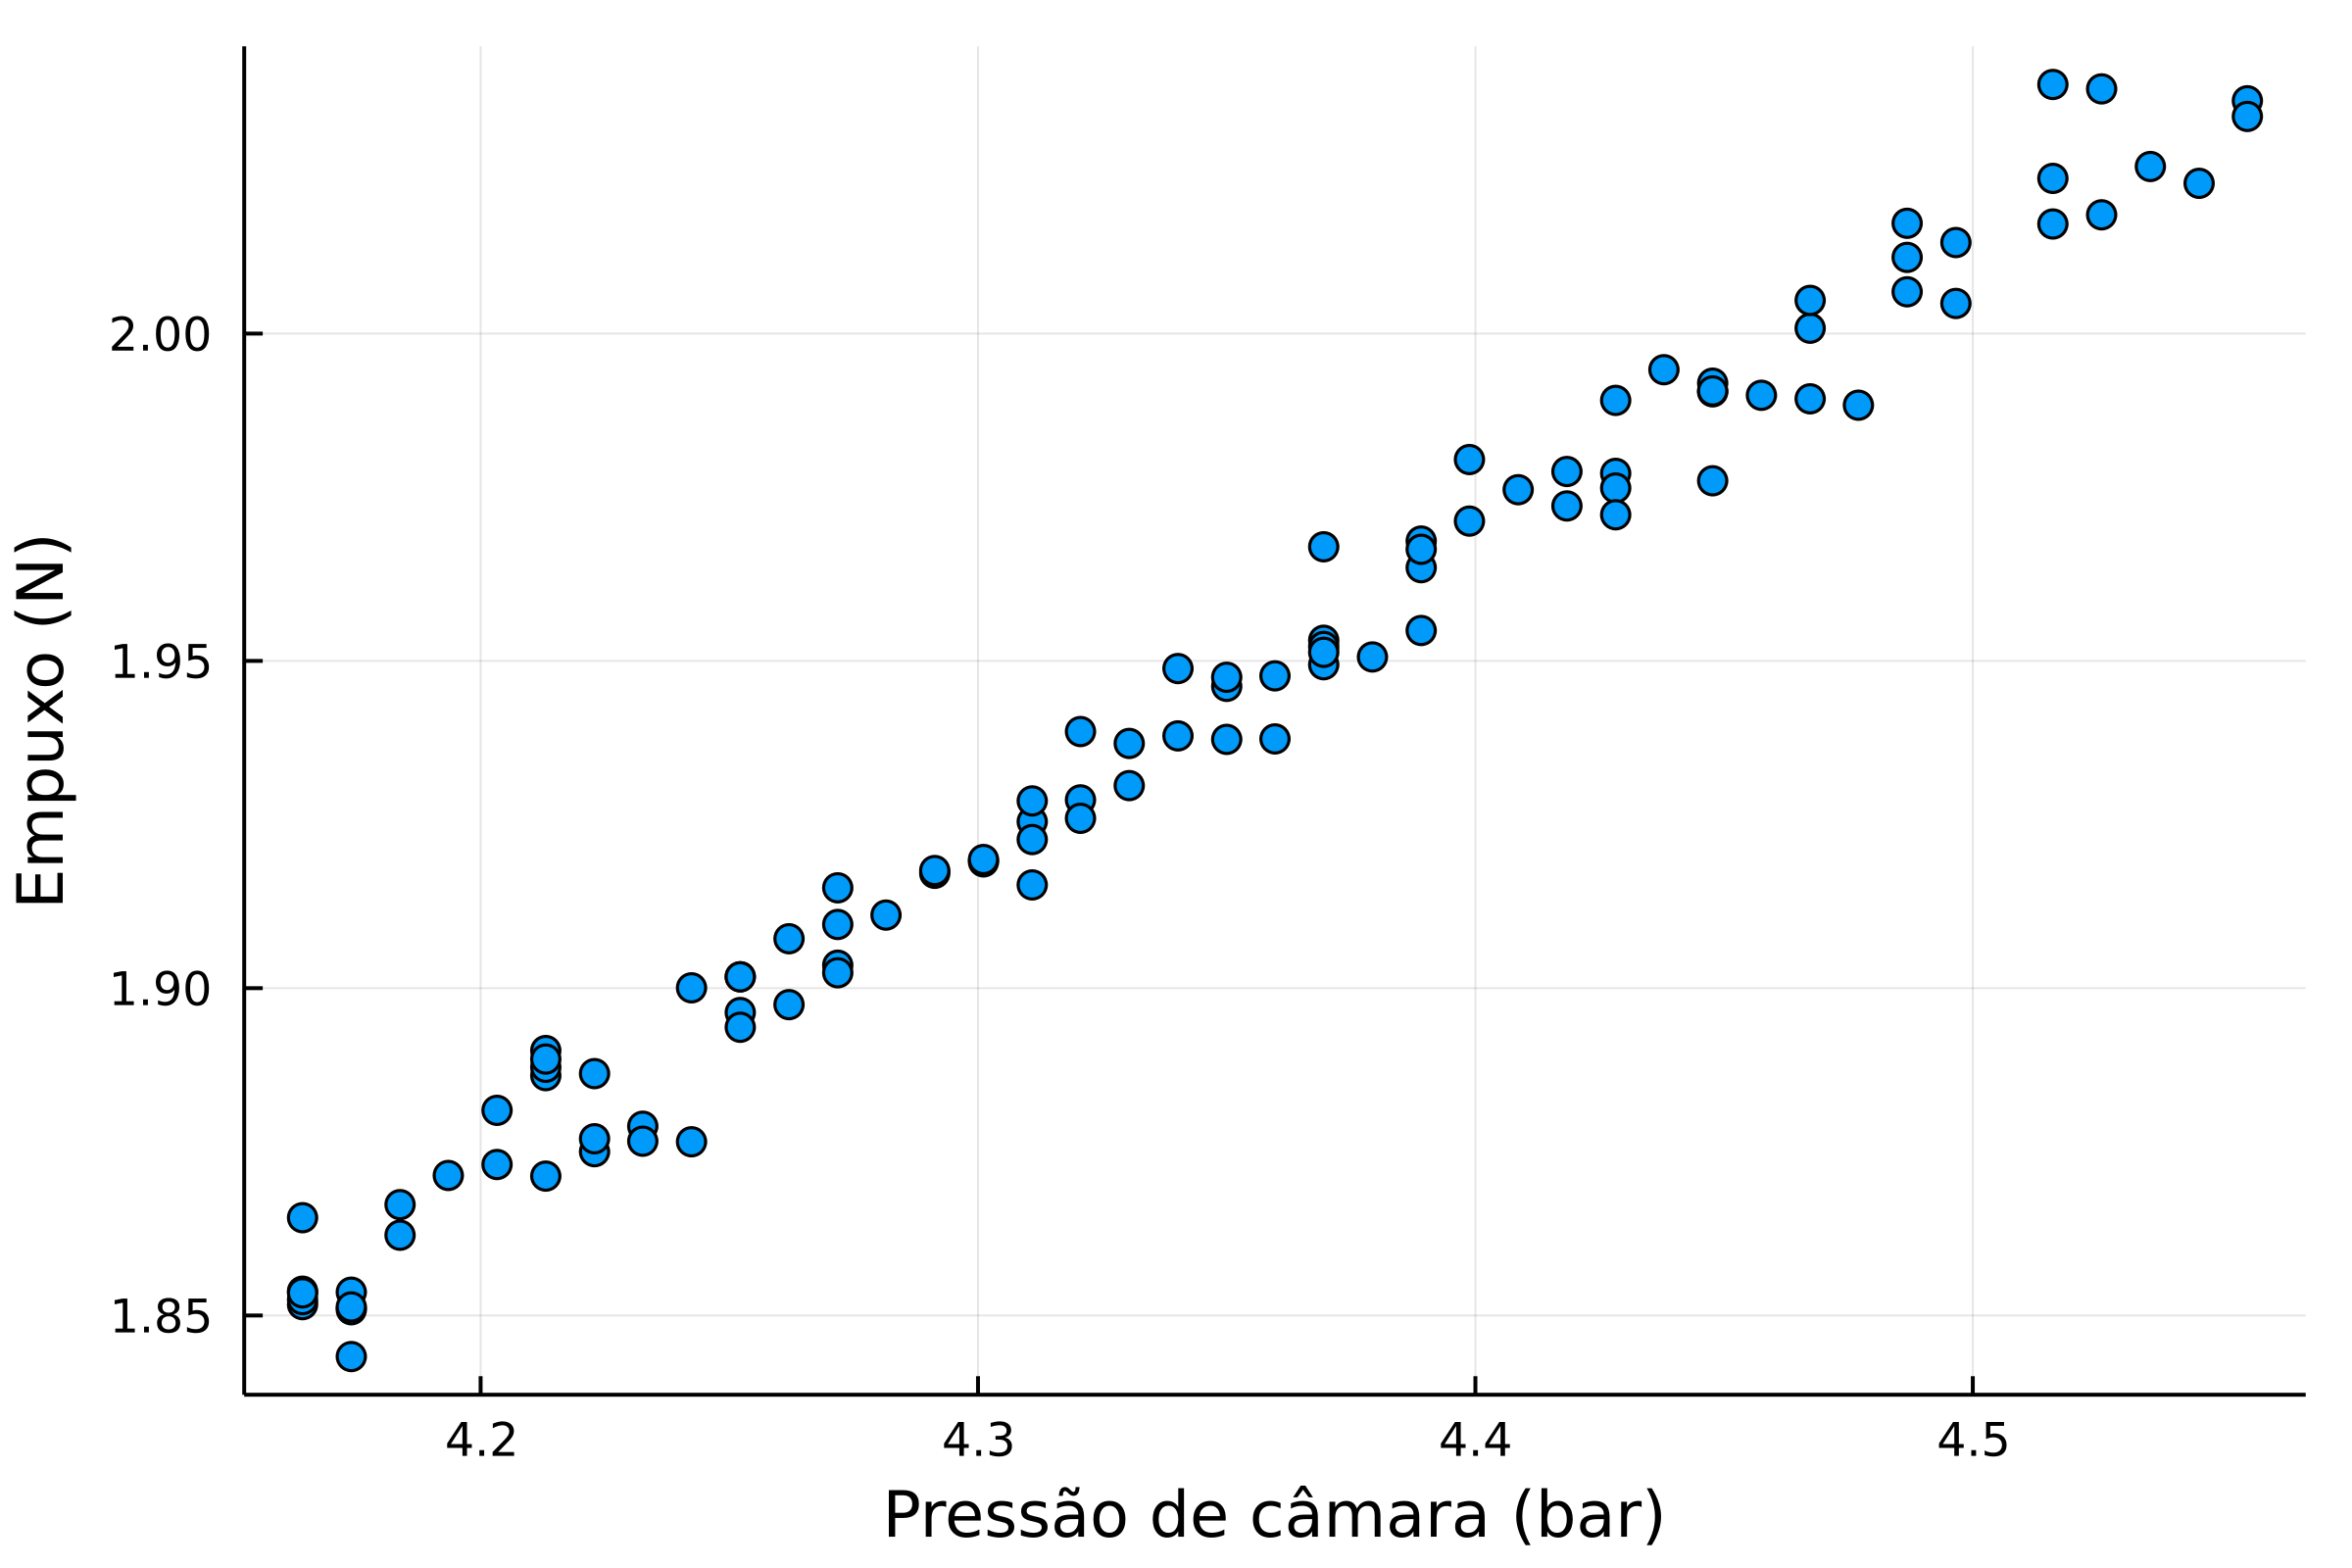
\includegraphics[width=\textwidth]{img/thrust_vs_chamber_pressure.png}
    \caption{Empuxo em função de pressão de câmara estática.}
    \label{fig:thrust_versus_p1}
\end{figure}

A variação de pressão de câmara observada neste ensaio deve-se ao grande fluxo mássico exigido pelo motor, de modo que houve esvaziamento significativo do compressor de ar utilizado durante o teste. Também destaca-se que a pressão medida na câmara, entre \(4,2bar\) e \(4,6bar\), foi inferior à pressão regulada em válvula, de exatamente \(5bar\). No entanto, o fato do motor real atingir os \(2N\) de empuxo exigidos com pressão próxima de \(4,5bar\) permitiu que a pesquisa continuasse levando-se em consideração as diferenças entre o motor real e o motor projetado.

Parâmetros propulsivos reais podem ser obtidos dos dados apresentados na figura~\ref{fig:thrust_versus_p1} através das equações~\ref{eq:C_F} e~\ref{eq:cstar}. Seus valores médios, com incerteza \(1\sigma \) são apresentados a seguir. A \(2N\) de empuxo, obteve-se impulso específico de \(46,6s\).
\begin{align}
    C_F &= 1,228 \pm 0,005 \\
    C^* &= (368,8 \pm 2,4)\;\mathrm{m}\,\mathrm{s}^{-1}
\end{align}

\section{Projeto do sistema de \textit{jet vanes}}

A montagem projetada de acordo com o método descrito na seção~\ref{sec:method_jet_vanes} está exibida em fotografias de quatro vistas nas figuras.

\section{Caracterização do sistema em balança de três componentes}